%\begin{myillus}

		Courbe représentative de la fonction $f(x) = \sqrt{x}$ et tableau de variations associé:
	\begin{multicols}{2}

	


	\begin{center}
		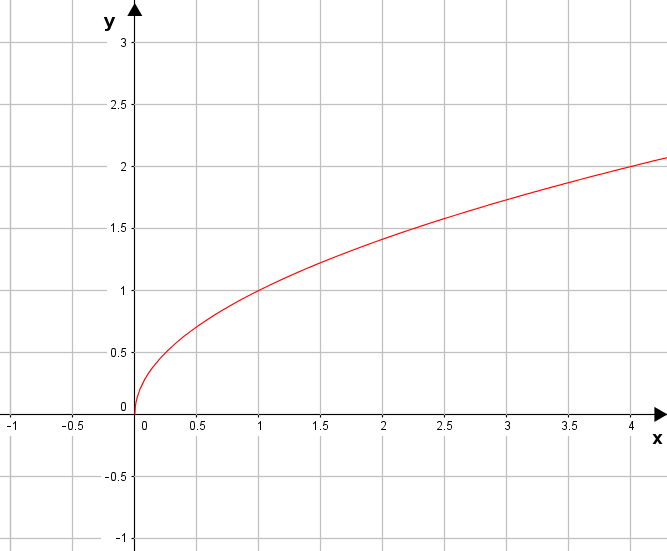
\includegraphics[scale=0.6]{./img/racine}
	\end{center}
	
	

	\vspace*{1cm}
	\begin{center}
%		\begin{tikzpicture}
%		\tkzTabInit{$x$/1,$f(x)$/2}{$- \infty$,$0$,$+ \infty$}
%		%\tkzTabLine{,-,z,+}
%		\tkzTabVar{+/$+ \infty$,-/$0$,+/$+ \infty$}
%		\end{tikzpicture}	

	\begin{variations}
		x & 0 & &  & & \pI \\
		\filet
		\sqrt{x} & & + &  \\				
	\end{variations}

	\vspace*{0.5cm}

		\begin{variations}
			x & & 0 & & \pI \\
		\filet
			\m{\sqrt{x}} & & \ & \c & \h\ \\				
		\end{variations}
	\end{center}
	\end{multicols}
%\end{myillus}